% Reliable Pairwise Preference Modeling for LLM Responses
% ACL format. Compile: tectonic report.tex   (or pdflatex + bibtex, or upload the folder to Overleaf)
\documentclass[11pt]{article}
\usepackage[final]{acl}
\usepackage{times}
\usepackage{latexsym}
\usepackage[T1]{fontenc}
\usepackage[utf8]{inputenc}
\usepackage{microtype}
\usepackage{inconsolata}
\usepackage{graphicx}
\usepackage{booktabs}
\usepackage{multirow}
\usepackage{amsmath}
\usepackage{xcolor}

\newcommand{\sym}{\textsc{sym}}
\newcommand{\pa}{p_{A}}

\title{Accuracy Is Not Enough: Position Bias, Length Bias and Calibration\\
in Pairwise Preference Models for LLM Responses}

\author{Ashish Sinha \\
  Indian Institute of Technology Bhilai \\
  \texttt{ashishsinha@iitbhilai.ac.in}}

\begin{document}
\maketitle

\begin{abstract}
Pairwise preference models decide which of two LLM responses a human would prefer; they are the reward models of RLHF and the judges of automatic evaluation. They are usually compared by accuracy alone. We build a cascade of preference models, from a length-only baseline through TF-IDF, BiLSTM, BERT and DeBERTa-v3 cross-encoders and a bi-encoder to a few-shot LLaMA-3-8B judge, and audit them for position bias, length bias, calibration, agreement with human vote distributions and domain shift. On Anthropic HH-RLHF, a 184M-parameter DeBERTa ensemble beats the 8B LLM judge by 4.7 points (66.5\% vs.\ 61.9\%) and is far better calibrated (ECE 0.04 vs.\ 0.31). Every cross-encoder changes its decision on 14--23\% of pairs when the two responses are swapped; training-time swap augmentation does not fix this for transformers, while averaging both orders at inference restores consistency and adds 1 point of accuracy. All architectures prefer the longer of two same-content answers 59--68\% of the time. On Stanford Human Preferences, training on vote shares instead of majority labels reduces calibration error 3--4.5$\times$ and the divergence from human vote distributions by 36--60\% at every model size, without hurting accuracy; post-hoc temperature scaling matches soft labels on top-label calibration but not on the vote distribution. Neither MC dropout nor deep ensembles detect pairs on which humans disagree, and helpfulness-trained models fall below chance on harmlessness prompts.
\end{abstract}

\section{Introduction}

Preference models are trained on pairs of responses to the same prompt with a human judgement of which is better \citep{christiano2017deep,stiennon2020learning}. They supply the reward signal for RLHF \citep{ouyang2022training,bai2022training}, are optimized implicitly by direct preference methods \citep{rafailov2023direct}, and are increasingly replaced or complemented by prompted LLM judges \citep{zheng2023judging}. Benchmarks rank them by pairwise accuracy \citep{lambert2024rewardbench}. Accuracy, however, says nothing about whether a model's decision depends on the order in which the responses are shown, whether it rewards length rather than content, whether its probabilities can be trusted, or whether it knows when humans themselves disagree. Each of these failure modes propagates into whatever system the preference model supervises.

We therefore treat a preference model as an instrument to be audited. We ask three research questions:
\textbf{RQ1} Can a small fine-tuned encoder predict human preferences as well as a much larger prompted LLM judge?
\textbf{RQ2} How sensitive are preference models to non-content factors (presentation order and response length), and which mitigations work?
\textbf{RQ3} Does training on annotator vote distributions (soft labels) instead of majority labels improve calibration and agreement with human disagreement?
We additionally test whether model uncertainty flags human disagreement and how models transfer across domains and label sources.

Our contributions are: (1) a single evaluation protocol applied to seven model tiers, with paired-bootstrap significance tests for every comparison; (2) evidence that position bias in cross-encoders is not removed by swap augmentation but is removed, with an accuracy gain, by symmetrizing predictions at inference, and that a bi-encoder is order-invariant at no accuracy cost; (3) a controlled length-perturbation test showing a persistent preference for longer same-content answers in all architectures; (4) evidence that soft labels improve calibration and distributional agreement at every model size, together with the finding that temperature scaling recovers top-label calibration but not distributional agreement; and (5) negative results: model uncertainty does not track human disagreement, and helpfulness and harmlessness preferences are anti-correlated across domains.

\section{Related Work}

\paragraph{Preference and reward models.}
Reward models are usually trained with a Bradley--Terry objective \citep{bradley1952rank} on human comparisons \citep{christiano2017deep,stiennon2020learning,ouyang2022training}. HH-RLHF \citep{bai2022training} is the standard public source of such comparisons; RewardBench \citep{lambert2024rewardbench} evaluates reward models by accuracy across categories. We complement accuracy with bias, calibration and disagreement measurements.

\paragraph{Biases of automatic judges.}
LLM judges favour a particular response position and longer responses \citep{zheng2023judging,wang2023large}, and LLMs are sensitive to option order more generally \citep{pezeshkpour2023large}. Length correlations pervade RLHF reward models \citep{singhal2023long}, motivating length-controlled evaluation \citep{dubois2024length}. We measure the same biases for small fine-tuned models and compare mitigations.

\paragraph{Calibration, uncertainty and disagreement.}
Modern neural networks are overconfident and can be recalibrated post hoc with temperature scaling \citep{guo2017calibration} or isotonic regression \citep{zadrozny2002transforming}. MC dropout \citep{gal2016dropout} and deep ensembles \citep{lakshminarayanan2017simple} estimate predictive uncertainty. Training on soft labels that reflect annotator disagreement can improve robustness and calibration \citep{peterson2019human,uma2021learning}. We test these ideas on preference data with real vote distributions \citep{ethayarajh2022understanding}, and compare human with AI-generated preference labels \citep{cui2024ultrafeedback}.

\section{Data}
\label{sec:data}

\paragraph{HH-RLHF} \citep{bai2022training}. We split each chosen/rejected dialogue into the shared prompt (up to the last assistant turn) and the two final responses, dropping 119 pairs without a shared prefix. The three \emph{helpful} subsets give 111,311 training, 5,997 validation and 6,194 test pairs; validation is split by prompt, and 33 training pairs whose prompt occurs in the test set are removed. The 44,729 \emph{harmless-base} pairs serve as an out-of-domain test set; for the reverse direction we split them by prompt into 38,741 / 1,995 / 3,993 pairs. Each pair has one human label.

\paragraph{Stanford Human Preferences (SHP)} \citep{ethayarajh2022understanding} contains 385K pairs of Reddit comments to the same post in 18 subreddits. We use the upvote share $\pa = s_A/(s_A+s_B)$ as a soft label. Training pairs pass a quality gate ($|s_A-s_B|>10$, $s_A+s_B>20$, $2|\pa-0.5|\geq0.2$; 37.9\% pass; at most five pairs per post), giving 72,216 pairs. The 18,406-pair test set is \emph{not} gated, so that 3,744 high-disagreement pairs ($0.4<\pa<0.6$, 20.3\%) remain for evaluation.

\paragraph{UltraFeedback} \citep{cui2024ultrafeedback}. For an AI-label ablation we use the binarized GPT-4-judged comparisons, drop ties, and keep 51,344 / 2,000 / 1,715 pairs, with soft target $\sigma(\text{score}_A-\text{score}_B)$.

\paragraph{Preprocessing.} In every dataset the preferred response is placed in position A or B uniformly at random (seed 42), so labels carry no position information. All transformer inputs share one token budget: \texttt{[CLS]} prompt \texttt{[SEP]} A \texttt{[SEP]} B \texttt{[SEP]}, keeping the last 128 prompt tokens and the first 190 tokens of each response. With the DeBERTa tokenizer, 7.1\% of HH and 18.6\% of SHP training responses exceed the response budget.

\paragraph{Human length preference.} Humans prefer the longer response in 55.8\% of HH-helpful pairs and 68.5\% of gated SHP pairs (62.8\% on the ungated test set), but only 42.0\% of HH-harmless pairs (Figure~\ref{fig:eda} in the appendix). A length-only model is therefore a strong baseline on helpfulness data and a misleading one on harmlessness data.

\section{Models}
\label{sec:models}

All models output $\pa$, the probability that response A is preferred.

\paragraph{T0: Length only and TF-IDF.} Logistic regression on the log length ratio $\log\frac{|A|+1}{|B|+1}$, and on the difference of TF-IDF vectors of the two responses (10K uni- and bigrams). Neither has an intercept, so both are order-invariant by construction.

\paragraph{T1: BiLSTM.} A two-layer bidirectional LSTM \citep{hochreiter1997long} with attention pooling (10.7M parameters, trained from scratch on the BERT WordPiece vocabulary), either over the concatenated input (\emph{cross}) or applied separately to (prompt, A) and (prompt, B) with $\text{logit}=s(A)-s(B)$ (\emph{siamese}).

\paragraph{T2/T3: Cross-encoders.} BERT-base \citep{devlin2019bert} (110M) and DeBERTa-v3-base \citep{he2023debertav3} (184M) read the full input; a linear layer on the \texttt{[CLS]} state gives the logit. Both responses attend to each other, which also allows the model to learn a position preference.

\paragraph{T5: Bi-encoder.} A shared BERT-base scores \texttt{[CLS]} prompt \texttt{[SEP]} response \texttt{[SEP]} for each response separately and $\pa=\sigma(s(A)-s(B))$, the standard reward-model design \citep{ouyang2022training}, as in Siamese sentence encoders \citep{reimers2019sentence}. Swapping A and B exactly negates the logit.

\paragraph{T6: LLM judge.} LLaMA-3-8B-Instruct \citep{dubey2024llama}, not fine-tuned, is shown the conversation and both responses with three HH-training examples whose answers alternate A, B, A, and asked which response is better (prompt in Appendix~\ref{app:prompts}). $\pa$ is the softmax over the next-token logits of ``A'' and ``B''.

\paragraph{Training.} Neural models minimize binary cross-entropy against the hard label or the soft target $\pa$. Transformers use AdamW (learning rate $2\times10^{-5}$, weight decay 0.01, 10\% warmup, linear decay), an effective batch of 32 and at most three epochs, with validation every 1,000 steps and early stopping on validation loss (patience 3), which selects the best-calibrated checkpoint. BERT trains in bf16; DeBERTa-v3 trains in fp32 because bf16 autocast produced NaN predictions. Hyperparameters are listed in Appendix~\ref{app:hparams}. Main runs use seed 42; deep ensembles add seeds 1 and 2. Total compute was about 35 GPU-hours on one RTX 6000 Ada.

\section{Evaluation Protocol}
\label{sec:eval}

\paragraph{Accuracy and calibration.} We report accuracy (with 95\% bootstrap intervals), AUC, NLL, and expected calibration error (ECE) over the confidence of the predicted winner (15 bins on $[0.5,1]$). On SHP we also report the Bernoulli KL divergence from the human vote share to the prediction, $\mathrm{KL}(\pa^{\text{human}}\,\|\,\pa^{\text{model}})$, overall and on the high-disagreement subset.

\paragraph{Swap test (position bias).} Every pair is scored in both orders. \emph{Swap consistency} is the fraction of pairs whose decision follows the swap; \emph{position bias} is the mean of $p_{AB}+p_{BA}-1$ (positive values favour the first slot). \emph{Symmetrization} averages the two orders, $p_{\sym}=(p_{AB}+1-p_{BA})/2$.

\paragraph{Test B (length perturbation).} From 500 HH test pairs whose chosen response has 40--150 words, Qwen2.5-7B-Instruct \citep{qwen2024qwen25} rewrites the chosen response to be about 40\% shorter while keeping its content (achieved median length ratio 0.46). We evaluate five variants with randomized order: the original pair; the compressed chosen response against the rejected one; the rejected response padded with two content-free sentences; and two unlabelled same-content pairs (original vs.\ compressed, original vs.\ padded), on which we measure how often the model picks the longer version.

\paragraph{Calibration and uncertainty.} Temperature scaling, isotonic regression and symmetrization are fitted on each model's own validation set. MC dropout uses 10 stochastic passes; deep ensembles average the logits of three seeds. We measure with AUROC whether the spread across passes or members, or low confidence $|\pa-0.5|$, identifies errors and high-disagreement SHP pairs.

\paragraph{Significance.} Comparisons on the same test pairs use a paired bootstrap with 2,000 resamples \citep{efron1994introduction}; we report the difference, its 95\% interval and a two-sided $p$-value (Appendix~\ref{app:significance}).

\section{Results}

\begin{table*}[t]
\centering
\small
\resizebox{\textwidth}{!}{\begin{tabular}{llrcccccc}
\toprule
Tier & Model & Params & Accuracy [95\% CI] & Acc.\ \sym & AUC & ECE & Swap cons. & Harmless \\
\midrule
T0 & Length only & 1 & 55.6 [54.3, 56.8] & 55.6 & .590 & .020 & .98 & 42.2 \\
T0 & TF-IDF + LR & 10K & 60.3 [59.1, 61.6] & 60.3 & .656 & .016 & 1.00 & 38.5 \\
T1 & BiLSTM cross & 11M & 61.7 [60.6, 62.9] & 62.2 & .676 & .024 & .78 & 37.3 \\
T1 & BiLSTM siamese & 11M & 63.0 [61.9, 64.3] & 63.0 & .686 & .012 & 1.00 & 36.1 \\
T2 & BERT cross & 110M & 63.6 [62.4, 64.8] & 64.6 & .706 & .022 & .77 & 35.2 \\
T2 & BERT cross, 3-seed ensemble & 330M & 64.4 [63.2, 65.8] & 65.1 & .714 & .024 & .82 & 34.6 \\
T5 & BERT bi-encoder & 110M & 64.6 [63.4, 65.9] & 64.6 & .711 & .023 & 1.00 & 34.3 \\
T3 & DeBERTa-v3 cross & 184M & 65.8 [64.6, 67.0] & 66.8 & .726 & .064 & .82 & 34.6 \\
T3 & DeBERTa-v3 cross, 3-seed ensemble & 552M & \textbf{66.5} [65.4, 67.7] & \textbf{67.5} & \textbf{.736} & .039 & .86 & 33.8 \\
T6 & LLaMA-3-8B judge, 3-shot & 8B & 61.9 [60.8, 63.1] & 63.6 & .670 & .313 & .60 & \textbf{52.6}$^\dagger$ \\
\bottomrule
\end{tabular}}
\caption{HH-RLHF helpful test set (6,194 pairs), all models trained on HH helpful. Acc.\ \sym: accuracy after averaging both presentation orders. Swap cons.: fraction of decisions that follow an A/B swap. Harmless: accuracy on the 44,729 harmless pairs ($^\dagger$1,000-pair random sample for the judge).}
\label{tab:main}
\end{table*}

\subsection{RQ1: Small fine-tuned models vs.\ an LLM judge}

Accuracy rises steadily with model capacity (Table~\ref{tab:main}, Figure~\ref{fig:ladder}): from 55.6\% for response length alone to 60.3\% for TF-IDF, 63.0\% for the best BiLSTM, 63.6\% for BERT and 65.8\% for DeBERTa-v3 (DeBERTa vs.\ BERT $+2.2$ points, $p=0.003$). Seeds vary by about $\pm0.5$ points (BERT 63.6/64.4/63.6, DeBERTa 65.8/66.2/66.4), and a three-seed DeBERTa ensemble reaches 66.5\%, or 67.5\% when symmetrized.

The few-shot LLaMA-3-8B judge reaches 61.9\%, between TF-IDF and the BiLSTM. The DeBERTa ensemble is 4.7 points more accurate (95\% CI [3.2, 6.1], $p<0.001$), and the gap remains 3.9 points when both models are symmetrized. The judge is also badly calibrated: ECE 0.313 against 0.039, and temperature scaling needs $T=11.1$ to reduce its ECE to 0.013. Its one advantage is robustness to domain shift (\S\ref{sec:shift}). \textbf{Answer to RQ1:} on in-distribution human preferences a fine-tuned 184M-parameter encoder is significantly more accurate and far better calibrated than an 8B prompted judge. Our initial target of 72\% accuracy was not reached by any model; HH labels come from a single annotator, which limits attainable accuracy.

\begin{figure}[t]
\centering
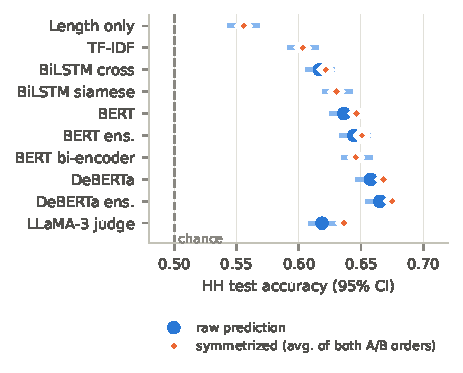
\includegraphics[width=\columnwidth]{figures/fig1_accuracy_ladder.pdf}
\caption{HH test accuracy by model with 95\% bootstrap intervals, before (circles) and after (diamonds) symmetrizing both presentation orders.}
\label{fig:ladder}
\end{figure}

\subsection{RQ2: Position and length bias}

\paragraph{Position.} Order-invariant models (length, TF-IDF, siamese BiLSTM, bi-encoder) are consistent under swaps by construction. Every model that reads both responses jointly is not (Figure~\ref{fig:swap}): the BiLSTM cross model and BERT follow the swap on only 77--78\% of pairs, DeBERTa on 82\%, and the LLM judge on 60\%, with a strong preference for the first response (position bias $+0.31$). Under domain shift the problem grows: SHP-trained BERT and DeBERTa follow the swap on only 43--46\% of HH pairs.

Training on randomly swapped copies (swap probability 0.5) raises the BiLSTM's consistency from 0.78 to 0.88 but barely changes the transformers (BERT 0.77$\to$0.79, accuracy $+0.8$ points, $p=0.10$; DeBERTa 0.82$\to$0.80). Symmetrizing at inference, in contrast, yields consistency 0.999 and \emph{improves} accuracy (BERT $+1.0$, $p=0.024$; DeBERTa $+1.1$, $p=0.009$), at the cost of a second forward pass. The bi-encoder is consistent by design and at least as accurate as the BERT cross-encoder ($+1.0$ points, $p=0.054$): cross-attention between the responses buys no accuracy on HH, only position sensitivity.

\begin{figure}[t]
\centering
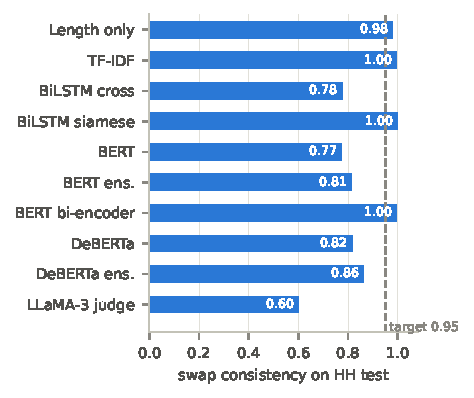
\includegraphics[width=\columnwidth]{figures/fig2_swap_consistency.pdf}
\caption{Swap consistency on HH test (1.0 = the decision never depends on presentation order); dashed line: the project's 0.95 target.}
\label{fig:swap}
\end{figure}

\paragraph{Length.} On HH test the correlation between length difference and the label is $r=0.11$ for humans, but 0.23--0.41 for the trained models (TF-IDF 0.41, BERT 0.35, DeBERTa 0.23) and 0.78 for the length-only model. Test B isolates the effect (Table~\ref{tab:testb}, Figure~\ref{fig:testb}). When the better answer is compressed to about half its length, accuracy drops by 3--7 points; given two versions of the same answer, every model prefers the longer one 59--68\% of the time. Content-free padding, by contrast, is not rewarded (41--55\%), so the bias is towards more \emph{content-bearing} text rather than towards more tokens. Accuracy on compressed pairs stays at 66--70\%, above the project's 65\% target. With 500 pairs, differences between models in Table~\ref{tab:testb} are within sampling error ($\pm4$ points). \textbf{Answer to RQ2:} position bias is large in joint-encoding models and is best removed at inference or by architecture; length bias persists in every architecture.

\begin{table}[t]
\centering
\small
\resizebox{\columnwidth}{!}{\begin{tabular}{lcccc}
\toprule
Model & Orig. & Compr. & Longer & Padded \\
\midrule
BERT cross & 75.2 & 68.0 & 66 & 41 \\
BERT + swap aug. & 71.2 & 68.0 & 59 & 50 \\
BERT no prompt & 73.0 & 69.6 & 61 & 44 \\
BERT bi-encoder & 74.2 & 67.2 & 68 & 44 \\
DeBERTa cross & 74.4 & 68.8 & 63 & 55 \\
DeBERTa + swap aug. & 73.0 & 65.6 & 63 & 48 \\
\bottomrule
\end{tabular}}
\caption{Test B on 500 HH pairs. Orig./Compr.: accuracy on the original pairs and with the preferred answer compressed to about half its length. Longer/Padded: \% of same-content pairs in which the model prefers the longer (uncompressed) or the filler-padded version; 50 = no preference.}
\label{tab:testb}
\end{table}

\begin{figure}[t]
\centering
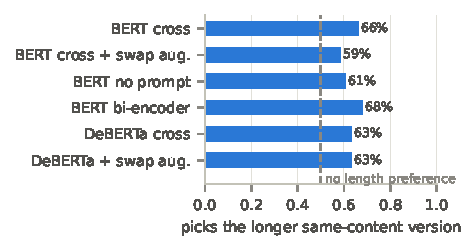
\includegraphics[width=\columnwidth]{figures/fig5_length_bias_test_b.pdf}
\caption{Share of same-content pairs in which each model picks the longer version (Test B).}
\label{fig:testb}
\end{figure}

\subsection{RQ3: Soft labels and calibration}

\begin{table}[t]
\centering
\small
\setlength{\tabcolsep}{4pt}
\resizebox{\columnwidth}{!}{\begin{tabular}{llccccc}
\toprule
& Labels & Acc. & ECE & KL & ECE$_{\text{HD}}$ & KL$_{\text{HD}}$ \\
\midrule
\multirow{3}{*}{BiLSTM} & hard & 66.3 & .068 & .206 & .102 & .183 \\
& hard + $T$ & 66.3 & .014 & .133 & .033 & -- \\
& soft & 66.6 & .021 & \textbf{.126} & .033 & \textbf{.063} \\
\midrule
\multirow{3}{*}{BERT} & hard & 68.0 & .062 & .205 & .098 & .189 \\
& hard + $T$ & 68.0 & .014 & .137 & .045 & .092 \\
& soft & \textbf{68.7} & .021 & \textbf{.131} & .046 & \textbf{.086} \\
\midrule
\multirow{3}{*}{DeBERTa} & hard & 69.9 & .109 & .339 & .153 & .384 \\
& hard + $T$ & 69.9 & .015 & .148 & .051 & .122 \\
& soft & 70.1 & .024 & \textbf{.137} & .048 & \textbf{.105} \\
\bottomrule
\end{tabular}}
\caption{SHP test set (18,406 pairs). Hard: trained on majority labels; hard + $T$: the same model after temperature scaling; soft: trained on vote shares. HD: the 3,744 high-disagreement pairs ($0.4<\pa<0.6$). KL: divergence from the human vote share.}
\label{tab:soft}
\end{table}

Table~\ref{tab:soft} and Figure~\ref{fig:reliability} compare training on majority labels with training on vote shares. At every tier, soft labels reduce ECE 3--4.5$\times$ (BiLSTM 0.068$\to$0.021, BERT 0.062$\to$0.021, DeBERTa 0.109$\to$0.024) and the KL divergence from human votes by 39\%, 36\% and 60\%, with even larger reductions on high-disagreement pairs (all $p<0.001$). Accuracy is unchanged or higher (BERT $+0.7$ points, $p=0.008$; BiLSTM and DeBERTa n.s.). The hard-label DeBERTa is the most overconfident model in the study (calibration temperature $T=1.91$); larger models overfit hard labels more.

The relevant baseline, however, is not the raw hard-label model but the same model after temperature scaling. Temperature scaling achieves slightly \emph{lower} top-label ECE than soft labels (BERT 0.014 vs.\ 0.021, $p=0.033$; DeBERTa 0.015 vs.\ 0.024, $p=0.008$), but soft labels remain significantly closer to the human vote distribution (KL 0.131 vs.\ 0.137 for BERT and 0.137 vs.\ 0.148 for DeBERTa; on high-disagreement pairs 0.086 vs.\ 0.092 and 0.105 vs.\ 0.122; all $p<0.001$). Soft-label models are slightly underconfident at the highest confidence levels (Figure~\ref{fig:reliability}). \textbf{Answer to RQ3:} soft labels improve calibration and distributional agreement at every model size; if only top-label calibration matters, temperature scaling is sufficient, but matching how humans split requires training on the split.

\begin{figure*}[t]
\centering
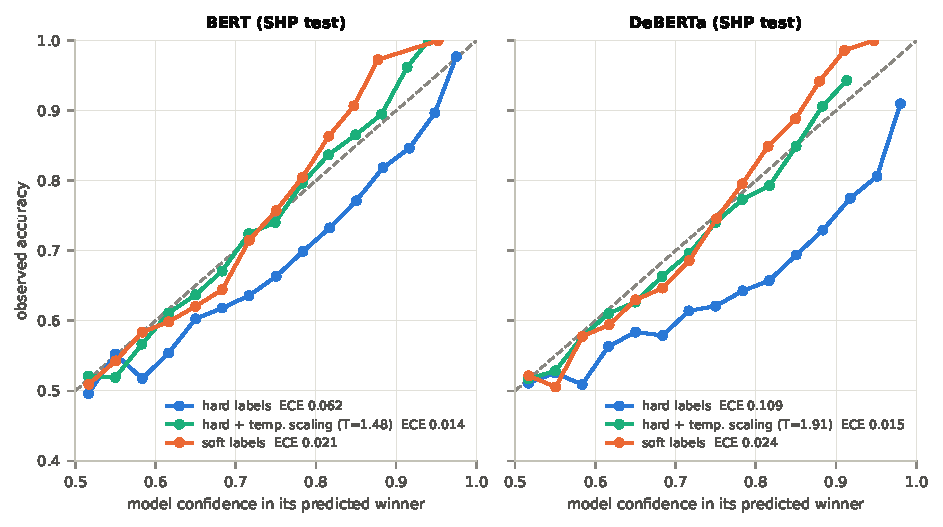
\includegraphics[width=\textwidth]{figures/fig3_reliability_shp.pdf}
\caption{Reliability diagrams on SHP test for BERT and DeBERTa trained on hard labels, the same models after temperature scaling, and models trained on soft labels. The dashed diagonal is perfect calibration.}
\label{fig:reliability}
\end{figure*}

\subsection{Does model uncertainty flag human disagreement?}

A practical use of uncertainty is to route ambiguous pairs to human review. We test whether MC dropout spread, ensemble spread, or low confidence identifies the 20.3\% of SHP test pairs on which voters split (Table~\ref{tab:uncertainty}). None does: AUROC is 0.50--0.51 for hard-label models and 0.52--0.54 for soft-label models, and flagging predictions in the 0.4--0.6 band raises the share of high-disagreement pairs only from 20.3\% to 21--22\%. Uncertainty is somewhat more informative about the model's own errors in domain (AUROC 0.58--0.59 for DeBERTa on HH; 0.62 for soft-label models on SHP). Model uncertainty and human disagreement are different quantities, and the former cannot stand in for the latter.

\begin{table}[t]
\centering
\small
\setlength{\tabcolsep}{4pt}
\resizebox{\columnwidth}{!}{\begin{tabular}{lccc}
\toprule
Model, method & Errors & HD (spread) & HD ($|\pa-.5|$) \\
\midrule
BERT hard, MC dropout & .506 & .503 & .508 \\
BERT hard, ensemble & .506 & .513 & .507 \\
DeBERTa hard, MC dropout & .502 & .499 & .509 \\
DeBERTa hard, ensemble & .520 & .496 & .499 \\
BERT soft, MC dropout & .621 & .523 & .539 \\
DeBERTa soft, MC dropout & .618 & .521 & .534 \\
\bottomrule
\end{tabular}}
\caption{AUROC on SHP test for detecting the model's errors and high-disagreement (HD) pairs from the spread across dropout passes or ensemble members, or from low confidence. 0.5 = no signal. Hard models were trained on HH, soft models on SHP.}
\label{tab:uncertainty}
\end{table}

\subsection{Domain shift and label source}
\label{sec:shift}

\begin{table}[t]
\centering
\small
\setlength{\tabcolsep}{3.5pt}
\resizebox{\columnwidth}{!}{\begin{tabular}{lcccc}
\toprule
Trained on $\downarrow$ / tested on $\rightarrow$ & Helpful & Harmless & SHP & UF \\
\midrule
HH helpful (human) & \textbf{63.6} & 35.0 & 55.0 & 50.4 \\
HH harmless (human) & 42.0 & \textbf{69.6} & 44.6 & 49.0 \\
SHP (human, soft) & 54.0 & -- & \textbf{68.7} & -- \\
UltraFeedback (GPT-4) & 55.2 & 44.7 & 57.8 & \textbf{65.7} \\
\bottomrule
\end{tabular}}
\caption{Transfer matrix for the BERT cross-encoder (accuracy). Harmless: the held-out harmless test split (3,993 pairs). UF: UltraFeedback test set.}
\label{tab:transfer}
\end{table}

Helpfulness-trained models score 34--42\% on harmlessness prompts, \emph{below} chance, and the stronger the model, the lower the score (length-only 42.2\%, DeBERTa ensemble 33.8\%; Figure~\ref{fig:shift} in the appendix). The reverse also holds: a model trained on harmless pairs reaches 69.6\% on harmless but 42.0\% on helpful prompts (Table~\ref{tab:transfer}). The two labelling criteria are not just different but opposed: on harmlessness prompts humans tend to prefer the shorter, refusing response, while helpfulness models learned to reward longer, more forthcoming answers. The LLM judge, which was never trained on either, is the only model above chance on harmless prompts (52.6\%).

Training on GPT-4 judgements (UltraFeedback) instead of human labels transfers slightly better to unseen human data (SHP 57.8\% vs.\ 55.0\% for the HH-trained model, $p<0.001$) but is much worse on HH human preferences (55.2\% vs.\ 63.6\%, $p<0.001$) and worse calibrated (ECE on HH 0.124 vs.\ 0.022). AI-generated preferences are not a drop-in substitute for in-domain human labels.

\subsection{Ablation: is the prompt used?}

A BERT cross-encoder that never sees the prompt is as accurate as the full model (63.7\% vs.\ 63.6\%, $p=0.88$). On HH, the model mostly judges response quality in isolation rather than whether a response fits its prompt. Because HH prompts are often generic, this result may not hold for tasks where correctness depends on the question.

\section{Discussion}

Three practical recommendations follow. \emph{First}, report swap consistency next to accuracy: a modest average position bias (BERT: $+0.06$) hides 23\% of decisions that flip with order, so part of a cross-encoder's accuracy rests on order-dependent decisions. Symmetrizing at inference or using a bi-encoder removes the problem without losing accuracy; augmentation alone does not. \emph{Second}, when vote distributions exist, train on them: soft labels give better-calibrated and more human-like probabilities at no cost. When they do not, temperature scaling repairs top-label calibration, including for LLM judges, whose raw probabilities are almost useless (ECE 0.31). \emph{Third}, do not use model uncertainty as a proxy for human disagreement, and do not assume a preference model transfers between helpfulness and harmlessness: the two are anti-correlated, which argues for separate or conditioned reward models.

Length bias is the one failure we could not mitigate. Every architecture prefers longer same-content answers even though the human length correlation on HH is small ($r=0.11$). Because the bias survives order-invariant architectures, augmentation and the removal of the prompt, it likely reflects the training labels' weak length preference amplified by the model, and calls for length-controlled objectives or counterfactual training data.

\section{Conclusion}

We audited preference models from a length baseline to an 8B LLM judge on accuracy, position bias, length bias, calibration, disagreement and domain shift. Small fine-tuned encoders are more accurate and much better calibrated than a prompted LLM judge on in-distribution data, but they inherit position and length biases that accuracy hides. Inference-time symmetrization, order-invariant architectures and soft-label training each fix a specific reliability problem; length bias and the gap between model uncertainty and human disagreement remain open.

\section*{Limitations}

Most configurations were trained with a single seed; the three-seed runs suggest seed variation of about $\pm0.5$ points, comparable to some reported differences. We used base-size encoders only: DeBERTa-v3-large was not trained because fp32 training would have required about a GPU-day. The 190-token response budget truncates 18.6\% of SHP responses, so some length differences are invisible to the encoders. SHP upvote shares are a proxy for annotator votes and are affected by comment timing and visibility. The Test B compressions were produced by an LLM and only spot-checked, and the test has 500 pairs. The LLM judge results cover one model, one prompt and three examples; its harmless and SHP numbers use 1,000-pair samples, and a frontier judge such as GPT-4 was not evaluated. HH labels come from a single annotator per pair, which caps attainable accuracy and prevents measuring disagreement there. No new human annotations were collected, and all data are English.

\section*{Ethics Statement}

HH-RLHF contains offensive and harmful content, including in its harmlessness subset; we used it only for training and evaluation, and the accompanying demo warns users before showing examples. All datasets are public and contain no personal information beyond public Reddit comments in SHP. Preference models trained on these data encode the values of their annotators and should not be deployed to judge content without review; our results on domain shift show how differently they behave outside their training distribution. Experiments used about 35 GPU-hours.

\bibliography{references}

\appendix

\section{Hyperparameters}
\label{app:hparams}

\begin{table}[h]
\centering
\small
\resizebox{\columnwidth}{!}{\begin{tabular}{lccc}
\toprule
& BiLSTM & BERT & DeBERTa-v3 \\
\midrule
Learning rate & $10^{-3}$ & $2\!\times\!10^{-5}$ & $2\!\times\!10^{-5}$ \\
Batch (effective) & 64 & 32 & 16$\times$2 \\
Max.\ epochs & 6 & 3 & 3 \\
Warmup & 5\% & 10\% & 10\% \\
Precision & fp32 & bf16 & fp32 \\
Early stopping & 2 epochs & 3 evals & 3 evals \\
Dropout & 0.3 & 0.1 & 0.1 \\
\bottomrule
\end{tabular}}
\caption{Training hyperparameters. All use AdamW with weight decay 0.01 and gradient clipping at 1.0; transformers are validated every 1,000 optimizer steps. The token budget is 128 prompt and 2$\times$190 response tokens. Bi-encoder: as BERT.}
\end{table}

\section{Prompts}
\label{app:prompts}

\paragraph{LLM judge.} System: \emph{``You are an expert evaluator of AI assistant responses. You will see a conversation between a human and an AI assistant, followed by two candidate final assistant responses, A and B. Decide which response is better.''} User: the conversation (last 300 words), Response A and Response B (first 250 words each), followed by \emph{``Which response is better? Answer with a single letter: A or B.''} Three HH training examples precede the query as user/assistant turns.

\paragraph{Test B compression.} \emph{``Rewrite the following response so that it is about 40\% shorter. Keep every piece of information, every instruction and the same tone. Do not add anything new. Output only the rewritten response.''} Padding appends two of six content-free sentences such as \emph{``I hope this helps!''} and \emph{``Let me know if you have any other questions.''}

\section{Significance Tests}
\label{app:significance}

\begin{table*}[t]
\centering
\small
\begin{tabular}{llrrrc}
\toprule
Comparison (A vs.\ B) & Metric & A & B & $\Delta$ [95\% CI] & $p$ \\
\midrule
DeBERTa ensemble vs.\ LLaMA-3 judge (HH) & accuracy & .665 & .619 & +.047 [+.032, +.061] & $<$.001 \\
DeBERTa ensemble vs.\ LLaMA-3 judge (HH) & ECE & .039 & .313 & $-$.273 [$-$.284, $-$.256] & $<$.001 \\
same, both symmetrized & accuracy & .675 & .636 & +.039 [+.025, +.053] & $<$.001 \\
DeBERTa vs.\ BERT (HH) & accuracy & .658 & .636 & +.022 [+.009, +.034] & .003 \\
BERT symmetrized vs.\ raw & accuracy & .646 & .636 & +.010 [+.002, +.019] & .024 \\
DeBERTa symmetrized vs.\ raw & accuracy & .668 & .658 & +.011 [+.003, +.018] & .009 \\
BERT swap augmentation vs.\ none & accuracy & .645 & .636 & +.008 [$-$.001, +.018] & .099 \\
BERT bi-encoder vs.\ cross-encoder & accuracy & .646 & .636 & +.010 [+.000, +.020] & .054 \\
BERT without vs.\ with prompt & accuracy & .637 & .636 & +.001 [$-$.008, +.009] & .877 \\
BERT soft vs.\ hard (SHP) & KL & .131 & .205 & $-$.073 [$-$.076, $-$.071] & $<$.001 \\
DeBERTa soft vs.\ hard (SHP) & KL & .137 & .339 & $-$.202 [$-$.206, $-$.197] & $<$.001 \\
BERT soft vs.\ hard + $T$ (SHP) & ECE & .021 & .014 & +.007 [+.001, +.014] & .033 \\
BERT soft vs.\ hard + $T$ (SHP) & KL & .131 & .137 & $-$.006 [$-$.008, $-$.005] & $<$.001 \\
DeBERTa soft vs.\ hard + $T$ (SHP) & ECE & .024 & .015 & +.009 [+.002, +.014] & .008 \\
DeBERTa soft vs.\ hard + $T$ (SHP) & KL & .137 & .148 & $-$.011 [$-$.013, $-$.010] & $<$.001 \\
Harmless- vs.\ helpful-trained, on harmless & accuracy & .696 & .350 & +.346 [+.321, +.370] & $<$.001 \\
Harmless- vs.\ helpful-trained, on helpful & accuracy & .420 & .636 & $-$.217 [$-$.236, $-$.196] & $<$.001 \\
GPT-4- vs.\ human-label training, on SHP & accuracy & .578 & .550 & +.028 [+.018, +.038] & $<$.001 \\
GPT-4- vs.\ human-label training, on HH & accuracy & .553 & .636 & $-$.084 [$-$.099, $-$.068] & $<$.001 \\
\bottomrule
\end{tabular}
\caption{Paired bootstrap tests (2,000 resamples) on identical test pairs. The full list, including all SHP metrics, is in \texttt{results/significance.csv}.}
\label{tab:significance}
\end{table*}

\section{Additional Figures}

\begin{figure}[h]
\centering
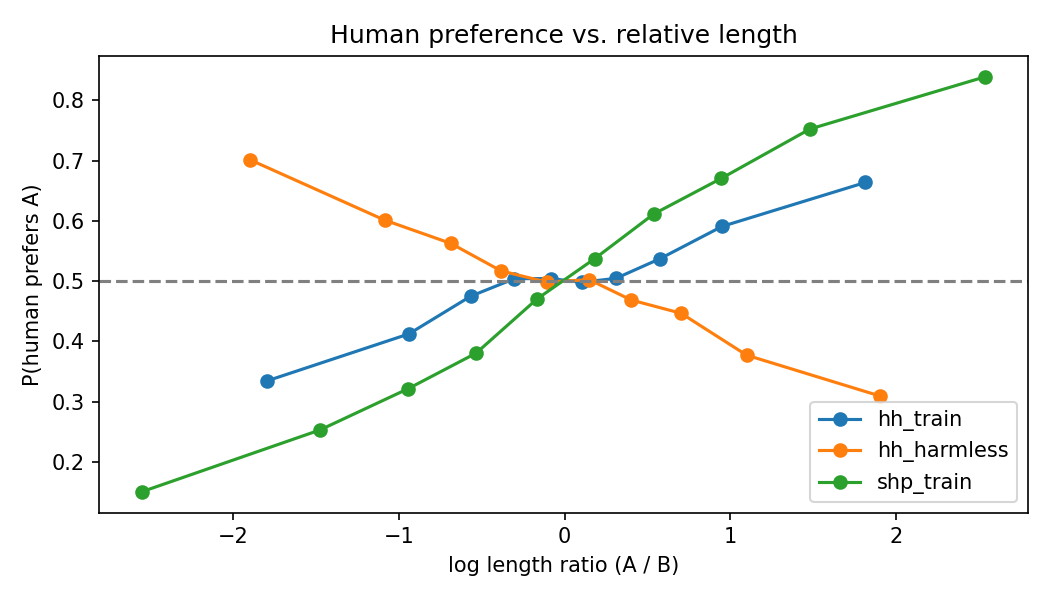
\includegraphics[width=\columnwidth]{figures/length_vs_preference.png}
\caption{Probability that humans prefer response A as a function of the log length ratio A/B (training sets). Humans prefer longer responses on HH helpful and SHP, but shorter ones on HH harmless.}
\label{fig:eda}
\end{figure}

\begin{figure}[h]
\centering
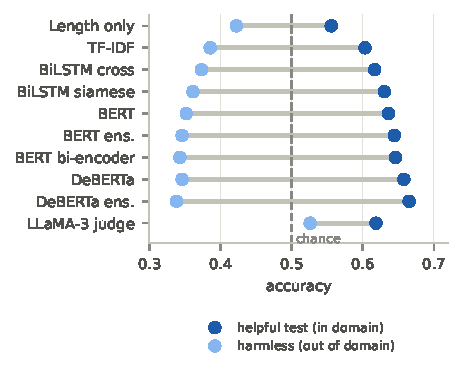
\includegraphics[width=\columnwidth]{figures/fig6_domain_shift.pdf}
\caption{Accuracy of HH-helpful-trained models on the helpful test set and on harmless prompts.}
\label{fig:shift}
\end{figure}

\begin{figure*}[h]
\centering
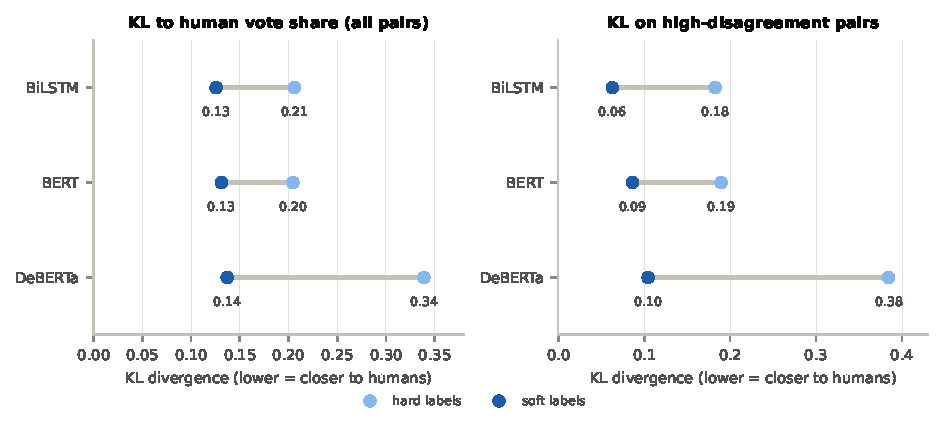
\includegraphics[width=\textwidth]{figures/fig4_rq3_kl_hard_vs_soft.pdf}
\caption{KL divergence from the human vote share on SHP test for hard- and soft-label models, on all pairs and on high-disagreement pairs.}
\label{fig:kl}
\end{figure*}

\end{document}
